\documentclass[11pt,a4paper]{article}
\usepackage[utf8]{inputenc}
\usepackage[T1]{fontenc}
\usepackage{charter}
\usepackage{amsmath,amssymb,amsthm}
\usepackage[margin=0.78in, top=0.82in, bottom=0.82in]{geometry}
\usepackage{graphicx,booktabs,tabularx,hyperref,xcolor,fancyhdr,microtype,caption}

\definecolor{primary}{RGB}{27, 79, 114}
\definecolor{accent}{RGB}{192, 57, 43}
\definecolor{graytext}{RGB}{90, 90, 90}

\hypersetup{colorlinks=true, linkcolor=primary, citecolor=primary, urlcolor=primary}
\setlength{\parskip}{4pt plus 1pt minus 1pt}
\setlength{\parindent}{0pt}

\pagestyle{fancy}
\fancyhf{}
\fancyhead[L]{\small\color{graytext}2026 MCM Senior Group Problem B: Scheduling a GPU Cluster}
\fancyhead[R]{\small\color{graytext}Team Submission Report}
\fancyfoot[C]{\small\thepage}
\renewcommand{\headrulewidth}{0.4pt}

\newcommand{\takeaway}[2]{%
  \vspace{4pt}%
  \noindent\colorbox{primary!7}{%
    \parbox{\dimexpr\textwidth-2\fboxsep\relax}{%
      \vspace{2pt}\textbf{\color{primary}#1:}\hspace{0.4em}#2\vspace{2pt}%
    }%
  }%
  \vspace{4pt}%
}

\newcommand{\QOneJobs}{224,112}
\newcommand{\QOneNodes}{4,278}
\newcommand{\QOneGpus}{10,412}
\newcommand{\QOneCpus}{632,636}
\newcommand{\QOneModels}{6}
\newcommand{\QOneHorizon}{7,775,878}
\newcommand{\QOneWindowDifference}{122}
\newcommand{\QOneOriginJobs}{3,512}
\newcommand{\QOneFractionalCpuJobs}{73}
\newcommand{\QOneZeroCpuJobs}{1}
\newcommand{\QOneMeanWorkers}{1.539}
\newcommand{\QOneMeanWorkerGpus}{2.003}
\newcommand{\QOneSingleWorkerPct}{90.95}
\newcommand{\QOneOneGpuPct}{78.42}
\newcommand{\QOneWorkMillion}{24.606}
\newcommand{\QOneGini}{0.9522}
\newcommand{\QOneDurationGini}{0.9580}
\newcommand{\QOneMedianDuration}{1,330}
\newcommand{\QOnePninetyfiveDuration}{309.09}
\newcommand{\QOneMaxDurationDays}{184}
\newcommand{\QOneHorizonHours}{2,159.966}
\newcommand{\QOnePhasePeak}{16}
\newcommand{\QOnePhaseTrough}{4}
\newcommand{\QOnePhaseRatio}{2.29}
\newcommand{\QOneTopPointOneCount}{224}
\newcommand{\QOneTopPointOneShare}{14.66}
\newcommand{\QOneTopOneCount}{2,241}
\newcommand{\QOneTopOneShare}{43.30}
\newcommand{\QOneTopFiveCount}{11,205}
\newcommand{\QOneTopFiveShare}{87.68}
\newcommand{\QOneAtenMean}{3,614.54}
\newcommand{\QOneAtenCapacity}{2,494}
\newcommand{\QOneAtenExcess}{1,120.54}
\newcommand{\QOneAtenPeak}{4,103}
\newcommand{\QOneAtenMeanPct}{144.93}
\newcommand{\QOneAtenRho}{2.064}
\newcommand{\QOneAhundredPeak}{2,922}
\newcommand{\QOneAtenCpu}{7.13}
\newcommand{\QOneRatioThreshold}{24}
\newcommand{\QOneHighRatioJobs}{2,478}
\newcommand{\QOneHighRatioPct}{25.70}
\newcommand{\QOneHighRatioWorkPct}{78.07}
\newcommand{\QOneOneSmallNodes}{1}
\newcommand{\QOneOneNodes}{901}
\newcommand{\QOneFourNodes}{10}
\newcommand{\QOneEightNodes}{77}


\usepackage{lastpage}
\begin{document}
\begin{titlepage}
\thispagestyle{fancy}
\begin{center}
\vspace*{0.35in}
{\LARGE\bfseries\color{primary} Evidence-Based Scheduling of a Heterogeneous GPU Cluster}\\[8pt]
{\large 2026 MCM Problem B}\\[12pt]
{\large Team Control Number: \ControlNumber}\\[18pt]
\end{center}
\takeaway{Submission identity}{Team members, institution, advisor, and final control number are intentionally not filled in this integration draft. The team must confirm them before submission.}
\section*{Summary}
This report studies a heterogeneous GPU cluster through three linked questions. First, the supplied 224,112-job trace is strongly concentrated: the GPU-work Gini coefficient is 0.9522, and the largest 5\% of jobs account for 87.68\% of GPU work. A10 has a lifetime-work/window-capacity ratio of 2.064 and a counterfactual immediate-start mean demand of 3,614.54 GPUs against 2,494 available; these are pressure diagnostics, not measured utilization.

Second, we evaluate capacity-valid, non-preemptive gang scheduling. On the complete 111,284-job A10 trace, ordinary \method{SPT-HOL} has mean waiting 32.906 h versus 34.967 h for \method{SPT-FILL}; the equal-weight GPU-count lower bound is 22.3179305700 h. A separate protected-policy comparison is limited to a verified 65,536-job prefix, where the added reservation policies remain substantially slower in mean waiting. These results support ordinary \method{SPT-HOL} as the current mean-wait candidate for this trace, without claiming dominance or no starvation.

Third, we evaluate a declared fixed-split cross-GPU substitution counterfactual. S0 routes a SHA-256-selected 10\% subset of A10 jobs to 60 dedicated A100 nodes with $\sigma=1$. It reduces A10 mean waiting from 900.129 to 587.875 h under FCFS and from 32.906 to 20.534 h under SJF-HOL, with zero additional native A100 waiting on this trace. The sensitivity study also finds that 20\% routing can worsen FCFS and 90 donor nodes cause measurable native harm. Compatibility and $\sigma$ are assumptions, not hardware benchmarks; unsupported resource-performance assertions are excluded.

\textbf{Keywords:} GPU scheduling; gang placement; heterogeneous resources; head-of-line blocking; fixed-split counterfactuals
\vfill
\textit{This is an integration draft. The team must complete the control number, human review, and final AI-use record before submission.}
\end{titlepage}
\setcounter{page}{2}
\begingroup
% 11.1 TeX points keeps body/caption glyphs above 11 PDF points after conversion.
\renewcommand{\normalsize}{\fontsize{11.1pt}{13.3pt}\selectfont}
\normalsize
\captionsetup{font=normalsize}
\section{Question 1: Data Characteristics and Resource Imbalance}
\label{sec:q1}
\subsection{Data Characteristics}
The competition's adapted Alibaba trace contains \QOneJobs{} jobs and \QOneNodes{} nodes, providing \QOneGpus{} GPUs and \QOneCpus{} vCPUs across \QOneModels{} models. Required fields have no missing values or duplicate identifiers. We retain fractional CPU requests. Each job $j$ has submission time $r_j$, duration $d_j$ (seconds), and $W_j$ identical workers, each requesting $g_j$ GPUs and $c_j$ vCPUs. Requests are per worker; multiplying by $W_j$ gives the whole-job demand. Node capacities are treated as fixed. The supplied records contain requests rather than measured hardware activity; GPU names alone do not identify training, inference or application compatibility.

Most jobs are small by worker count: \QOneSingleWorkerPct\% have one worker, and \QOneOneGpuPct\% request one GPU per worker; the corresponding means are \QOneMeanWorkers{} and \QOneMeanWorkerGpus{}. Duration is highly dispersed: the median is \QOneMedianDuration{} s, the 95th percentile \QOnePninetyfiveDuration{} h, and the maximum approximately \QOneMaxDurationDays{} days. Thus a typical job poorly represents the long-duration tail.

Define full-lifetime GPU work as $H_j=W_jg_jd_j$ in GPU-seconds; $H_j/3600$ gives GPU-hours. Total work is \QOneWorkMillion{} million GPU-hours, with empirical Gini \QOneGini{}. Using $k=\lfloor f|\mathcal{J}|\rfloor$, the top 1\% (\QOneTopOneCount{} jobs) and 5\% (\QOneTopFiveCount{}) account for \QOneTopOneShare\% and \QOneTopFiveShare\% of work. Figure~\ref{fig:q1} shows concentration and duration tails; neither establishes a fitted power law. Queueing experiments must test whether these large jobs obstruct smaller arrivals.

\begin{figure}[!ht]
\centering
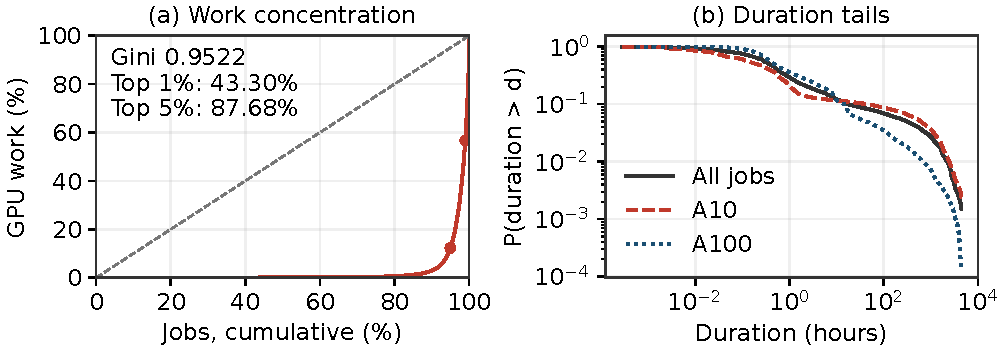
\includegraphics[width=\textwidth]{fig1_data_patterns.pdf}
\caption{(a) GPU-work Lorenz curve, including the origin; top-$k$ counts use floor rounding. (b) Strict empirical duration CCDF, $\Pr(d_j>x)$, with ties grouped; terminal zero is omitted on log axes. A100 denotes A100-SXM4-80GB.}
\label{fig:q1}
\end{figure}

\subsection{Supply--Demand Imbalance}
Set $T=\max_j r_j=\QOneHorizon$ s (\QOneHorizonHours{} h), \QOneWindowDifference{} s short of nominal 90 days. For model $m$, compare all submitted lifetime work with its capacity over $[0,T)$:
\begin{equation}
\rho_m^{\mathrm{GPU}}=\frac{\sum_{j\in\mathcal{J}_m}W_jg_jd_j}{T\sum_{i\in\mathcal{I}_m}G_i^{\mathrm{cap}}},\qquad
\rho_m^{\mathrm{CPU}}=\frac{\sum_{j\in\mathcal{J}_m}W_jc_jd_j}{T\sum_{i\in\mathcal{I}_m}C_i^{\mathrm{cap}}}.
\label{eq:load_ratio}
\end{equation}
Both denominators use seconds, matching the numerators. Work extending beyond $T$ remains included. These ratios measure workload pressure, not observed utilization or proof of steady-state instability. Table~\ref{tab:q1_pool} identifies A10's disproportionate pressure.

\begin{table}[!ht]
\centering
\caption{Submitted lifetime work versus exact-window capacity. Work is in million GPU-hours; GPU-s1/s2 abbreviate GPU-series-1/2.}
\label{tab:q1_pool}
\label{tab:q1_summary} % Preserve references from the integration baseline.
\setlength{\tabcolsep}{5pt}
\begin{tabular}{lrrrrr}
\toprule
GPU model & GPUs & Jobs & Work (10$^6$ GPU-h) & $\rho^{GPU}$ & $\rho^{CPU}$\\
\midrule
\texttt{A10} & 2,494 & 111,284 & 11.119 & 2.064 & 0.391\\
\texttt{A100-SXM4-80GB} & 3,456 & 80,877 & 5.936 & 0.795 & 0.534\\
\texttt{GPU-series-1} & 1,558 & 9,643 & 3.892 & 1.156 & 0.590\\
\texttt{H800} & 1,752 & 4,716 & 2.203 & 0.582 & 0.540\\
\texttt{GPU-series-2} & 976 & 13,633 & 1.224 & 0.580 & 0.382\\
\texttt{A800-SXM4-80GB} & 176 & 3,959 & 0.232 & 0.611 & 0.527\\
\textbf{Total} & 10,412 & 224,112 & 24.606 & 1.094 & 0.473\\
\bottomrule
\end{tabular}

\end{table}

To distinguish lifetime work from window overlap, define counterfactual immediate-start demand:
\begin{equation}
D_m(t)=\sum_{j\in\mathcal{J}_m}W_jg_j\mathbf{1}\{r_j\leq t<r_j+d_j\},\qquad
\overline{D}_m=\frac{1}{T}\int_0^T D_m(t)\,dt.
\label{eq:q1_demand}
\end{equation}
This assumes submission-time starts and ignores capacity. Exact event integration gives A10 a mean of \QOneAtenMean{} GPUs against \QOneAtenCapacity{} available, with an instantaneous peak of \QOneAtenPeak{}. The mean excess of \QOneAtenExcess{} GPUs is not a sufficient expansion prescription: CPU, node placement and temporal overlap also matter. Lower mean demand elsewhere does not guarantee spare capacity at every instant.

\begin{figure}[!ht]
\centering
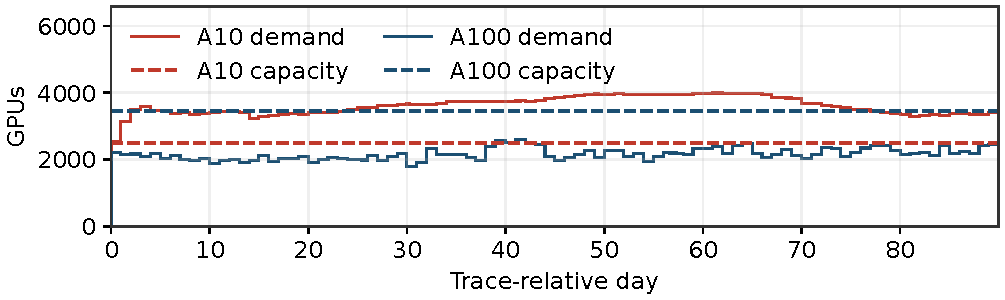
\includegraphics[width=\textwidth]{fig1_demand.pdf}
\caption{Counterfactual immediate-start demand, displayed as exact daily overlap averages. Dashed lines show physical capacity. Daily averaging hides instantaneous peaks; these curves are not actual allocation.}
\label{fig:q1-demand}
\end{figure}

All nodes are initially idle. The \QOneOriginJobs{} submissions at $r_j=0$ are the trace-origin batch, not already running services. Excluding that batch, exposure-corrected arrival rates differ by \QOnePhaseRatio{} times between relative 24-hour phases \QOnePhasePeak{} and \QOnePhaseTrough{}. With no calendar origin or timezone, these phases cannot identify afternoon or night peaks. Supplementary plots show daily arrivals, submitted work and the full phase profile. Work grouped by submission day includes each job's entire future duration; it is not work executed that day.

\subsection{Bottleneck Hypotheses}
GPU-series-1 contains \QOneOneNodes{} nodes with $(1\text{ GPU},192\text{ vCPUs})$, \QOneOneSmallNodes{} with $(1,128)$, \QOneFourNodes{} with $(4,192)$, and \QOneEightNodes{} with $(8,192)$. A pool-average CPU/GPU ratio obscures these configurations. Exactly \QOneHighRatioJobs{} jobs (\QOneHighRatioPct\%; \QOneHighRatioWorkPct\% of pool work) exceed the 8-GPU nodes' \QOneRatioThreshold{} vCPU/GPU ratio. One 192-vCPU, 1-GPU worker can exhaust such a node's CPUs while leaving seven GPUs unavailable to positive-CPU workers. This illustrates a possible placement mechanism, not a measured schedule.

The evidence motivates testing head-of-line blocking, node-ratio-aware placement and explicitly compatible cross-model capacity. Questions 2--3 must evaluate waiting, allocation and fairness with capacity-valid schedules. Q1 supports these hypotheses, but proves neither their causal effects nor any scheduler's optimality.
\par\endgroup

% Canonical standalone Question 2 section.  The surrounding document_en.tex is
% an integration draft; this file is the Q2-only deliverable.
\section{Question 2: Capacity-Valid Scheduling and Method Selection}

\subsection{Model and policy definitions}
Each GPU model is evaluated as its own pool. Job $j$ has release time $r_j$,
duration $p_j$, $w_j$ workers, per-worker GPU request $g_j$, and CPU request
$c_j$. It starts at $s_j\ge r_j$, finishes at $s_j+p_j$, and all workers
start together. A placement is feasible only when, on every selected node $i$,
\[
g_jx_{j,i}\le G_i^{\rm free}(t),\qquad
c_jx_{j,i}\le C_i^{\rm free}(t),\qquad \sum_i x_{j,i}=w_j .
\]
The simulator is non-preemptive, uses exact integer-second durations, and
commits a gang placement atomically. All comparisons use the same numeric
First-Fit-by-ID (FF-id), raw CSV, loader ordering, and explicit
\texttt{shared-timer} event mode.

Ordinary \texttt{SPT-HOL} orders arrived jobs by
$(p_j,r_j,\mathrm{job\_id})$. It has no aging threshold, urgent promotion, or
reservation; if its head is infeasible, that dispatch epoch stops. Ordinary
\texttt{SPT-FILL} uses the same order but may inspect later feasible jobs. Its
\(K=200\) is a per-pool, per-timestamp budget only after a blocking prefix has
been encountered: feasible prefix checks do not consume it, successful and
failed bypass attempts both consume it, retries may consume it again, and a
successful start does not reset the timestamp budget. Shared timer ticks give
additional dispatch opportunities and can therefore change the observed
budgeted fill behavior. These statements describe only the tested
\(K=200\), FF-id, shared-timer configuration; they do not establish behavior
for an unbounded FILL policy. Ordinary \texttt{SPT-HOL} has no aging protection.

The formal A10 runs use $\theta=604800$ seconds (168 hours), $K=200$,
\texttt{shared-timer}, $H=7,776,000$ seconds, and complete drain. The threshold
is exploratory, not an optimum, and is an experiment configuration separate
from ordinary \texttt{SPT-HOL}. Protected urgent policies are reported only
for the verified 65,536-job A10 prefix.

\subsection{Job-count lower bound and exact waiting accounting}
For A10, let $C=2494$, $G_j=w_jg_j$, and
\[
Z(t)=\{j:r_j\le t<r_j+p_j\}.
\]
Let $q(t)$ be the minimum number of jobs removed from $Z(t)$ so that the
remaining GPU width is at most $C$. Then
\[
L_{\rm count}=\frac{1}{3600N}\int q(t)\,dt
\]
is a valid lower bound on ordinary mean waiting. The integral uses exact
half-open event intervals and integer GPU-width histograms. If $S(t)$ is the
actual service set, define $A(t)=S(t)\cap Z(t)$. A delayed job may still run
after $r_j+p_j$, so $S(t)\subseteq Z(t)$ is false in general. However,
$Z(t)\setminus A(t)$ is a deletion set leaving a feasible GPU total, so it has
at least $q(t)$ jobs. Therefore
\[
\sum_j\min(W_j,p_j)\ge\int q(t)\,dt,\qquad
\sum_jW_j\ge\int q(t)\,dt.
\]
The tuple $(r,p,s)=(0,2,4)$ illustrates the correction: at $t=5$ the job is
in $S(t)$ but not in $Z(t)$. Non-preemption gives the exact bookkeeping
identity $W_j=\min(W_j,p_j)+\max(W_j-p_j,0)$. The resulting three terms are
accounting around a relaxation, not causal shares or an exact distance to OPT.

\subsection{Complete A10 evidence}
The complete A10 input has 111,284 jobs and 2,494 nodes. The verified Q2 G2
SPT-HOL timing and the Q3 M0 SJF-HOL A10 timing have identical 111,284-row
ID, attribute, start, and finish records (canonical timing hash
\texttt{378acdbf...18baea8}). The full-cluster table below is read-only Q3
M0 FCFS/SJF-HOL evidence retrieved from fixed submission
\texttt{79e93c315f006d67f743b14a1d7faf16b00dd072}; its recorded run source is
commit \texttt{7075317883808b1cd7f80cadf3980be291c69cf0}. It is not a claim that the
Q2 engine ran a new 224,112-job trace.

\begin{table}[htbp]
\centering\small
\caption{Read-only Q3 M0 full-cluster summary, $H=90$ days; waiting uses complete drain.}
\begin{tabular}{llrrrrr}
\toprule
Policy & Pool & $n$ & Mean $W$ (h) & P95 (h) & Max (h) & $f\le H$\\
\midrule
FCFS & A10 &111284&900.129&1408.478&1423.254&54531\\
FCFS & A100-SXM4-80GB &80877&0.000&0.000&0.000&80101\\
FCFS & A800-SXM4-80GB &3959&0.146&0.000&12.250&3943\\
FCFS & GPU-series-1 &9643&0.029&0.000&9.971&8221\\
FCFS & GPU-series-2 &13633&0.045&0.000&6.992&13606\\
FCFS & H800 &4716&0.016&0.000&7.856&4705\\
FCFS & ALL &224112&446.971&1356.501&1423.254&165107\\
SJF-HOL & A10 &111284&32.906&11.087&3017.288&107002\\
SJF-HOL & A100-SXM4-80GB &80877&0.000&0.000&0.000&80101\\
SJF-HOL & A800-SXM4-80GB &3959&0.115&0.000&14.858&3943\\
SJF-HOL & GPU-series-1 &9643&0.434&0.000&76.818&8213\\
SJF-HOL & GPU-series-2 &13633&0.016&0.000&7.165&13606\\
SJF-HOL & H800 &4716&0.016&0.000&7.856&4705\\
SJF-HOL & ALL &224112&16.362&0.689&3017.288&217570\\
\bottomrule
\end{tabular}
\end{table}

For the A10 group, the job-count lower bound is
$8,941,062,908$ job-seconds, or $22.3179305700$ h. The Q1 fixed-pool
GPU-work-weighted lower bound is $560.5213678903$ h. With fixed
$H_j=w_jg_jp_j$ weights, the three persisted A10 timings give:

\begin{table}[htbp]
\centering
\caption{Ordinary and GPU-work-weighted A10 waiting; the two objectives need not rank policies alike.}
\begin{tabular}{lrrr}
\toprule
Policy & Mean job wait (h) & $\sum H_jW_j/\sum H_j$ (h) & Mean / job-count LB\\
\midrule
FCFS &900.129&619.352&40.33\\
SPT-HOL &32.906&677.690&1.47\\
SPT-FILL&34.967&677.496&1.57\\
\bottomrule
\end{tabular}
\end{table}

Thus SPT-HOL is the current ordinary-mean candidate, while the weighted
objective reverses the FCFS versus SPT ordering in this trace. Neither metric
alone establishes general optimality. The lower bound is conservative because
it relaxes CPU, node shape, and gang placement.

\subsection{Bounded protected-policy analysis and method choice}
On the verified 65,536-job A10 prefix, the ordinary means are 30.332 h
(SPT-HOL) and 31.042 h (SPT-FILL). URGENT-HOL/TIME/FIXED/FLEX are respectively
556.492/350.528/350.088/349.715 h; FIXED/FLEX accepted 62/133 crossings.
These are prefix protection-cost results only, not full-cluster or full-A10
urgent results. The FILL G3 cost record has 314,756 order builds. The
cross-review supplied 307,844 budget-exhausted events, giving 97.804% of
order-build records, but that ratio is a candidate-attempt diagnostic, not
97.804% of waiting time; the G3 archive does not independently persist that
event count.

For ordinary mean waiting, SPT-HOL is the current main candidate. SPT-FILL is
retained as a useful immediate-start baseline, and protected policies remain
valid safety or tail-preference experiments. SPT-HOL still has harmed jobs and
a slightly larger maximum wait than FILL; no dominance or general starvation
guarantee is claimed. All source hashes, row/ID checks, derived summaries,
and missing external full-cluster timing retention are recorded in
\texttt{results/20261016-b-q2-m2g-revision-01/}. The surrounding integrated
paper remains a draft; this file is the canonical Q2-only section.

\begingroup
\renewcommand{\normalsize}{\fontsize{11.1pt}{13.3pt}\selectfont}
\normalsize
\section{Question 3: Fixed-Split Cross-GPU Substitution}
\label{sec:q3}

\subsection{Model and assumptions}
We study a finite, whole-card, pre-start substitution policy on the supplied trace of 224,112 jobs. Job $j$ has native GPU model $n_j$, actual execution model $m_j$, duration $p_j$, worker count $W_j$, per-worker GPU request $g_j$, and per-worker CPU request $c_j$. A compatibility indicator $K_{jm}$ and multiplier $\sigma_{jm}$ are declared scenario assumptions; they are not measured hardware facts. For the only foreign edge in this study, A10 jobs may execute on A100-SXM4-80GB and
\begin{equation}
 p'_j=\sigma_{jm}p_j,
 \qquad f_j=s_j+p'_j,
 \qquad \omega_j=s_j-a_j.
\end{equation}
The fixed partition reserves the first $B$ A100 nodes in ascending `node_name` order for routed A10 jobs and leaves the other A100 nodes for native A100 jobs. Each worker's CPU and GPU remain on one physical node, all workers of a job start together, jobs are non-preemptive and non-migrating, and no resource may be used twice. At every node $i$ and time $t$,
\begin{equation}
 \sum_{j:s_j\le t<f_j}g_jy_{ji}\le G_i^{\rm cap},\qquad
 \sum_{j:s_j\le t<f_j}c_jy_{ji}\le C_i^{\rm cap},\qquad
 \sum_i y_{ji}=W_j.
\end{equation}
The model is a deterministic scheduling heuristic, not an optimality claim.

\subsection{Fixed-split counterfactual design}
M0 is the original model-isolated schedule. S0 is the earlier Q3-S1 M1 result, renamed to make the comparison unambiguous: 60 dedicated A100 nodes, a 10\% SHA-256 threshold, and $\sigma=1$. S1--S5 vary exactly one factor from S0: 5\% or 20\% routing, 30 or 90 donor nodes, or $\sigma=2$. The hash namespace is fixed as `q3-fixed-split-v1`; eligibility uses only the current job and declared capacity. There is no fallback from the foreign queue and no relocation of a running job.

We report $W=s-a$, actual JCT $J=f-a$, relative completion delay $f-a-p_j$, and paired finish difference $f_{\rm scenario}-f_{\rm reference}$. Every comparison uses the same original job IDs. The 90-day window is $H=7,776,000$ seconds; waiting and JCT use complete drain, while completion counts use $f_j\le H$.

\begin{table}[!ht]
\centering
\caption{Main Q3 results generated from the paper-ready JSON. Native harmed counts are paired against S0 under the same policy.}
\label{tab:q3_main}
\scriptsize
\begin{tabular}{llrrrrrr}
\toprule
Scenario & Policy & A10 $\bar W$ (h) & A10 P95/P99 (h) & A10 $\bar J$ (h) & Native harm & All $\bar J$ (h) & 90d done \\
\midrule
M0 & FCFS & 900.129 & 1408.478/1419.616 & 999.898 & 0 & 523.961 & 165,107 \
S0 & FCFS & 587.875 & 966.761/987.569 & 687.645 & 0 & 368.910 & 181,112 \
S1 & FCFS & 702.551 & 1167.986/1188.658 & 802.320 & 0 & 425.853 & 174,693 \
S2 & FCFS & 1010.136 & 4322.906/5345.115 & 1109.905 & 0 & 578.586 & 177,498 \
S3 & FCFS & 916.407 & 4053.782/4423.899 & 1016.177 & 0 & 532.044 & 174,139 \
S4 & FCFS & 539.109 & 958.246/985.841 & 638.878 & 5,735 & 344.723 & 184,339 \
S5 & FCFS & 721.752 & 2292.733/2885.707 & 831.456 & 0 & 440.320 & 177,166 \
M0 & SJF-HOL & 32.906 & 11.087/1542.181 & 132.676 & 0 & 93.353 & 217,570 \
S0 & SJF-HOL & 20.534 & 12.691/639.532 & 120.303 & 0 & 87.209 & 217,814 \
S1 & SJF-HOL & 25.328 & 7.745/1108.877 & 125.097 & 0 & 89.589 & 217,766 \
S2 & SJF-HOL & 22.058 & 9.767/526.165 & 121.827 & 0 & 87.965 & 218,104 \
S3 & SJF-HOL & 25.565 & 11.470/1025.261 & 125.334 & 0 & 89.707 & 217,762 \
S4 & SJF-HOL & 19.214 & 5.205/611.002 & 118.984 & 2,150 & 86.560 & 217,945 \
S5 & SJF-HOL & 25.106 & 12.125/1058.270 & 134.810 & 0 & 94.412 & 217,521 \
\bottomrule
\end{tabular}

\end{table}

\subsection{Benefit, native-pool cost and sensitivity}
With $\sigma=1$, S0 reduces A10 mean waiting from 900.129 to 587.875 hours under FCFS (34.7\% relative to M0) and from 32.906 to 20.534 hours under SJF-HOL (37.6\%). Cluster-wide mean JCT changes from 523.961 to 368.910 hours for FCFS and from 93.353 to 87.209 hours for SJF-HOL. The native A100 mean and P99 waiting costs are zero in S0 on this trace; this is a trace result, not an SLA.

More routing is not uniformly better. At 60 donor nodes, FCFS A10 mean waiting is 702.551, 587.875, and 1010.136 hours at 5\%, 10\%, and 20\%. The 20\% case is worse than both 10\% and M0. SJF-HOL gives 25.328, 20.534, and 22.058 hours, while its P99 tail and 90-day completion count move differently. These are finite fixed-split observations; they do not establish monotonicity for another trace or a dynamic policy.

At 10\% routing and $\sigma=1$, increasing donors from 30 to 60 to 90 lowers A10 mean waiting for both policies, but 90 nodes creates native A100 harm: 5,735 FCFS jobs and 2,150 SJF-HOL jobs wait longer than in S0. Their mean additional waits are 0.0771 and 0.0185 hours, respectively. The 90-node point remains in the trade-off table rather than being discarded.

\begin{figure}[!ht]
\centering
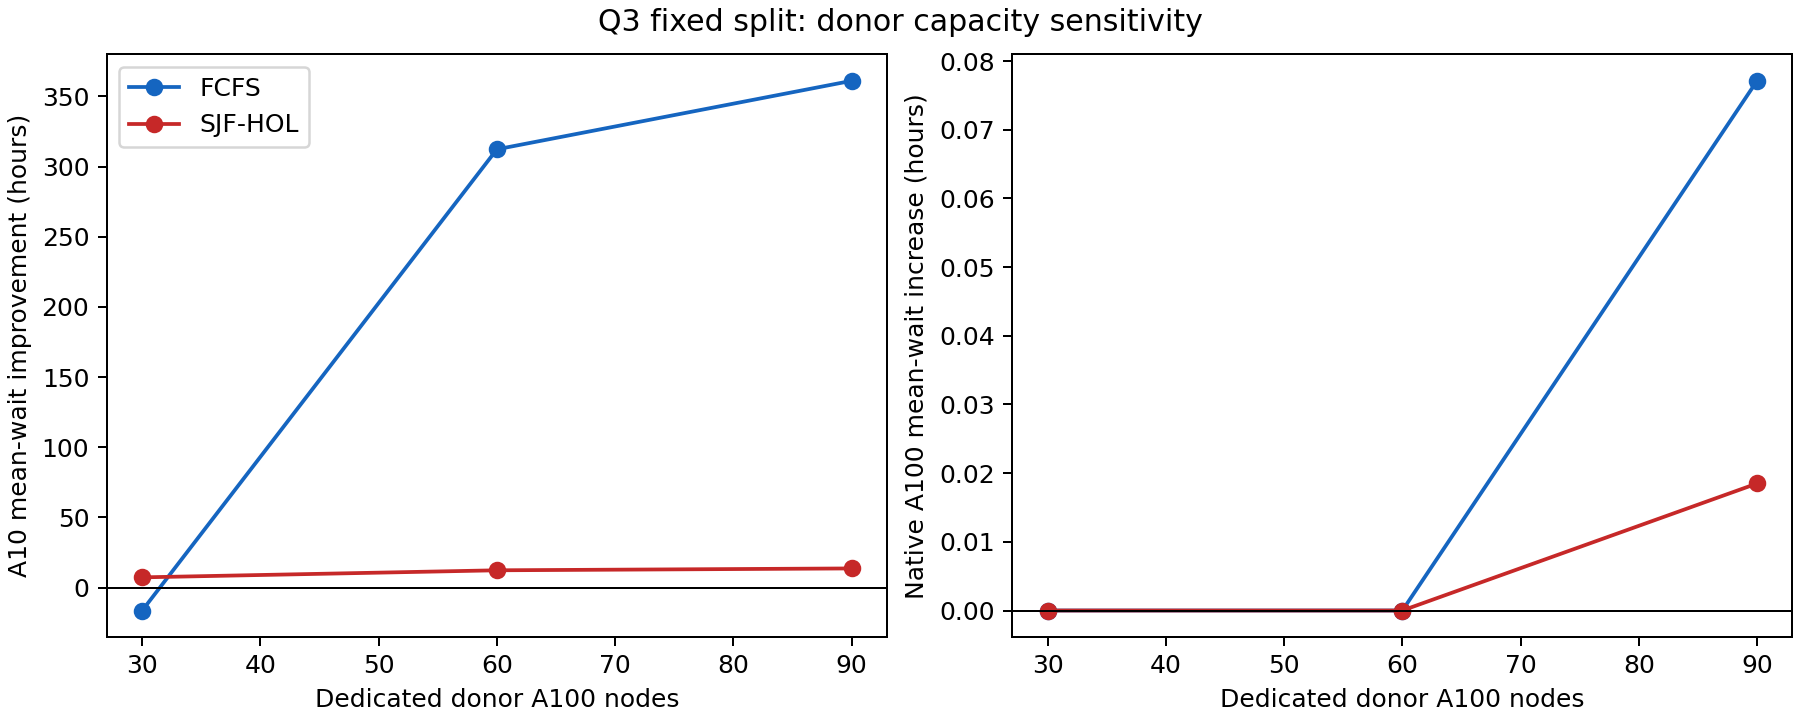
\includegraphics[width=\textwidth]{figures/q3_donor_capacity_wait_tradeoff.png}
\caption{Capacity sensitivity from the persisted S2 results. The left panel shows A10 mean-wait improvement relative to M0; the right panel shows native A100 mean-wait increase relative to M0. The two panels use different scales so the small native cost remains visible without being treated as zero.}
\label{fig:q3_capacity}
\end{figure}

For $\sigma=2$, the effective duration of routed A10 jobs doubles and SJF-HOL is re-simulated because its queue key changes. FCFS A10 mean JCT changes from 999.898 to 831.456 hours (paired delta -168.443 hours), while SJF-HOL changes from 132.676 to 134.810 hours (paired delta 2.134 hours). For the full trace, SJF-HOL all-job mean JCT changes from 93.353 to 94.412 hours and 90-day completions from 217,570 to 217,521; waiting falls relative to M0 but completion worsens. FCFS retains a mean-JCT benefit in this $\sigma=2$ scenario. No interpolation or exact break-even $\sigma^*$ is claimed.

\subsection{Conditional recommendation and limitations}
If the policy requirement is zero additional native A100 waiting on this trace, 60 nodes at 10\% is a tested candidate for either policy; it is not a proven maximum safe capacity or a global optimum. If a small native cost is acceptable, 90 nodes supplies an additional point on the A10--native trade-off. SJF-HOL's lower mean waiting does not remove its tail and completion-fairness losses; all harmed-job counts and positive delay totals remain in the paired evidence.

Compatibility and $\sigma$ are assumptions without an A10/A100 performance matrix. Allocation rates are request occupancy, not measured utilization; GPU-hours across models are not interchangeable compute or monetary units. The experiment adds no physical GPUs, does not implement dynamic sharing, MIG, pricing, RL, migration, or Q2\,$\times$\,Q3 scheduling, and does not prove heuristic optimality. Q1's A10 lower bound is not transferred to substituted schedules. The conclusion is therefore conditional on the declared trace, partitions, hash rule, policy, and duration scenarios.
\par\endgroup

\section{Conclusion and Evidence Limits}
\label{sec:conclusion}
The three questions provide complementary evidence rather than one universal scheduler claim. Q1 identifies workload concentration and two lower bounds with different weighting objectives. Q2 converts the diagnosis into a capacity-valid DES comparison: complete-A10 ordinary SPT-HOL is the current mean-wait choice, while protected policies are retained as bounded prefix experiments. Q3 evaluates a fixed, physical, pre-start substitution scenario and keeps both native-pool harm and duration sensitivity visible.

The reported numbers are separated by data set and horizon: Q1 uses the exact observation window $T=7,775,878$ s; scheduling metrics use complete drain; 90-day completion counts use $H=7,776,000$ s. Prefix evidence is never extended to the complete A10 trace without a corresponding saved run. The formal paper contains no unsupported performance, hardware-speed, or optimality claim. Large Q3 delivery archives are retained locally with hashes, but cross-machine availability remains unresolved.

\section*{References}
\sloppy
\begin{enumerate}[label={[\arabic*]}]
\item COMAP, \emph{2026 MCM Problem B: GPU Scheduling}, repository snapshot, fixed SHA256 \texttt{fb153a547ed57a3d16ab0929c27cccc5d49fc4e568d9c65a273546057e692967}.
\item Q1 capacity-bound evidence, repository commit \texttt{707531788380}; evidence path: \url{results/20261015-b-q1-capacity-bound/q1_capacity_bounds.json}. Full SHA is in \texttt{paper\_sources.json}.
\item Q2 cross-review evidence, repository commit \texttt{b91918bb08}; evidence paths: \url{results/20261016-b-q2-m2g-revision-01/} and \url{notes/tasks/b-q2.md}. Full SHA is in \texttt{paper\_sources.json}.
\item Q3 cross-review publication evidence, repository commit \texttt{170cc37a82}; evidence paths: \url{results/20261016-b-q3-s3-publication-9ac1d7f2-r3/} and \url{notes/tasks/b-q3.md}. Full SHA is in \texttt{paper\_sources.json}.
\item Claude independent research archive, stable ID \texttt{claude-p1p5-562e82aa}, archive commit \texttt{9aeddd708b}; full SHA and archive hash are in \texttt{paper\_sources.json}; used for provenance cross-reading only, not as a rerun.
\item COMAP, \emph{MCM/ICM Contest Rules, Registration and Instructions}, official online guidance: \url{https://contest.comap.org/undergraduate/contests/mcm/instructions.php}.
\end{enumerate}

\clearpage
\section*{Report on Use of AI Tools}
This section records the actual integration work and is pending team confirmation of the exact final disclosure wording. OpenAI Codex was used to inspect fixed Git commits, organize already saved Q1/Q2/Q3 evidence, draft and typeset this integration document, and run repository/PDF checks. The Claude package was treated as a preserved independent source; its scripts were not executed in this integration. No AI output is treated as experimental evidence without a fixed repository source and human review. Team members remain responsible for all mathematics, data interpretation, citations, source attribution, and final submission decisions.

\textbf{Team confirmation required:} verify the team control number, member/institution metadata, the exact AI product/model label required by the contest, and the final human review record before submission.
\end{document}
